\documentclass[12pt,a4paper]{book}
\usepackage[utf8]{inputenc}
\usepackage[english]{babel}
\usepackage{geometry}
\usepackage{graphicx}
\usepackage{float}
\usepackage{hyperref}
\usepackage{fancyhdr}
\usepackage{tocloft}
\usepackage{titlesec}
\usepackage{xcolor}
\usepackage{listings}
\usepackage{booktabs}
\usepackage{longtable}
\usepackage{array}
\usepackage{enumitem}
\usepackage{subcaption}

% Page geometry
\geometry{margin=2.5cm, headheight=15pt}

% Define Kanardia colors
\definecolor{kanardiaOrange}{RGB}{255,87,34}
\definecolor{kanardiaGray}{RGB}{102,102,102}
\definecolor{lightGray}{RGB}{245,245,245}

% Hyperlink setup
\hypersetup{
    colorlinks=true,
    linkcolor=kanardiaOrange,
    filecolor=magenta,      
    urlcolor=cyan,
    pdftitle={KanardiaCloud User Manual},
    pdfauthor={Kanardia d.o.o.},
    pdfsubject={Aviation Electronics and Cloud Services},
    pdfkeywords={Kanardia, Aviation, Electronics, Cloud, Flight Management}
}

% Header and footer
\pagestyle{fancy}
\fancyhf{}
\fancyhead[LE,RO]{\thepage}
\fancyhead[LO]{\rightmark}
\fancyhead[RE]{\leftmark}
\fancyfoot[C]{\textcolor{kanardiaGray}{KanardiaCloud User Manual}}

% Chapter and section formatting
\titleformat{\chapter}[display]
{\normalfont\huge\bfseries\color{kanardiaOrange}}
{\chaptertitlename\ \thechapter}{20pt}{\Huge}

\titleformat{\section}
{\normalfont\Large\bfseries\color{kanardiaOrange}}
{\thesection}{1em}{}

\titleformat{\subsection}
{\normalfont\large\bfseries\color{kanardiaGray}}
{\thesubsection}{1em}{}

% Code listings setup
\lstset{
    backgroundcolor=\color{lightGray},
    basicstyle=\footnotesize\ttfamily,
    breakatwhitespace=false,
    breaklines=true,
    captionpos=b,
    commentstyle=\color{kanardiaGray},
    deletekeywords={...},
    escapeinside={\%*}{*)},
    extendedchars=true,
    frame=single,
    keepspaces=true,
    keywordstyle=\color{kanardiaOrange},
    language=Python,
    morekeywords={*,...},
    numbers=left,
    numbersep=5pt,
    numberstyle=\tiny\color{kanardiaGray},
    rulecolor=\color{black},
    showspaces=false,
    showstringspaces=false,
    showtabs=false,
    stepnumber=1,
    stringstyle=\color{kanardiaOrange},
    tabsize=2,
    title=\lstname
}

% Define JSON language for listings
\lstdefinelanguage{json}{
    basicstyle=\normalfont\ttfamily,
    numbers=left,
    numberstyle=\scriptsize,
    stepnumber=1,
    numbersep=8pt,
    showstringspaces=false,
    breaklines=true,
    frame=single,
    backgroundcolor=\color{lightGray},
    literate=
     *{0}{{{\color{blue}0}}}{1}
      {1}{{{\color{blue}1}}}{1}
      {2}{{{\color{blue}2}}}{1}
      {3}{{{\color{blue}3}}}{1}
      {4}{{{\color{blue}4}}}{1}
      {5}{{{\color{blue}5}}}{1}
      {6}{{{\color{blue}6}}}{1}
      {7}{{{\color{blue}7}}}{1}
      {8}{{{\color{blue}8}}}{1}
      {9}{{{\color{blue}9}}}{1}
      {:}{{{\color{kanardiaOrange}{:}}}}{1}
      {,}{{{\color{kanardiaOrange}{,}}}}{1}
      {\{}{{{\color{kanardiaOrange}{\{}}}}{1}
      {\}}{{{\color{kanardiaOrange}{\}}}}}{1}
      {[}{{{\color{kanardiaOrange}{[}}}}{1}
      {]}{{{\color{kanardiaOrange}{]}}}}{1},
}

% Title page information
\title{
    \vspace{2cm}
    
\includegraphics[width=0.3\textwidth]{images/kanardia_logo.png}\\[2cm]
    {\Huge\bfseries KanardiaCloud}\\[0.5cm]
    {\Large User Manual}\\[1cm]
    {\large Version 1.0}
}
\author{Kanardia d.o.o.}
\date{\today}

\begin{document}

% Title page
\frontmatter
\maketitle

% Copyright page
\newpage
\thispagestyle{empty}
\vspace*{\fill}
\begin{center}
\textbf{Copyright Notice}\\[0.5cm]
\copyright\ 2025 Kanardia d.o.o. All rights reserved.\\[0.5cm]
This document contains proprietary and confidential information of Kanardia d.o.o.\\
No part of this document may be reproduced, distributed, or transmitted in any form\\
or by any means without the prior written permission of Kanardia d.o.o.\\[1cm]

\textbf{Contact Information}\\[0.5cm]
Kanardia d.o.o.\\
Dolenji Novaki pri Ajdovščini 14\\
5270 Ajdovščina, Slovenia\\[0.5cm]
Email: info@kanardia.com\\
Web: www.kanardia.com\\[1cm]

\textbf{Document Information}\\[0.5cm]
Document Version: 1.0\\
Last Updated: \today\\
Document Type: User Manual
\end{center}
\vspace*{\fill}

% Table of contents
\tableofcontents
\listoffigures
\listoftables

% Main content
\mainmatter

% Include chapters
\chapter{Introduction}

\section{About KanardiaCloud}

KanardiaCloud is a comprehensive cloud-based platform designed for aviation professionals and pilots. It provides a unified interface for managing flight-related data, including device synchronization, digital checklists, instrument layouts, logbook entries, and approach charts.

\subsection{Key Features}

\begin{itemize}[leftmargin=2cm]
    \item \textbf{Device Management}: Seamlessly sync with Kanardia avionics devices
    \item \textbf{Digital Checklists}: Create, manage, and print professional aviation checklists
    \item \textbf{Instrument Layouts}: Design custom instrument panel configurations
    \item \textbf{Electronic Logbook}: Comprehensive flight logging with automatic data synchronization
    \item \textbf{Approach Charts}: Store and organize airport approach procedures
    \item \textbf{Cloud Synchronization}: Real-time data sync across multiple devices
    \item \textbf{Multi-User Support}: Secure user authentication and data isolation
\end{itemize}

\subsection{System Requirements}

\begin{table}[H]
\centering
\begin{tabular}{@{}ll@{}}
\toprule
\textbf{Component} & \textbf{Requirement} \\
\midrule
Web Browser & Chrome 90+, Firefox 88+, Safari 14+, Edge 90+ \\
Internet Connection & Broadband connection required \\
Screen Resolution & 1024x768 minimum, 1920x1080 recommended \\
Operating System & Any modern OS with web browser support \\
JavaScript & Must be enabled \\
\bottomrule
\end{tabular}
\caption{System Requirements for KanardiaCloud}
\label{tab:system_requirements}
\end{table}

\subsection{Supported Devices}

KanardiaCloud is compatible with the following Kanardia aviation devices:

\begin{itemize}
    \item \textbf{NESIS III}: Advanced flight management system
    \item \textbf{NESIS IV}: Latest generation flight computer
    \item \textbf{KRT2 S}: VHF radio transceiver
    \item \textbf{KTX2}: Mode S transponder
    \item \textbf{Custom Integrations}: API support for third-party devices
\end{itemize}

\section{Getting Help}

\subsection{Documentation}
This user manual provides comprehensive information about all KanardiaCloud features. Each chapter includes:
\begin{itemize}
    \item Step-by-step instructions
    \item Screenshots and visual guides
    \item Best practices and tips
    \item Troubleshooting information
\end{itemize}

\subsection{Technical Support}
For technical support and assistance:

\begin{itemize}
    \item \textbf{Email}: support@kanardia.com
    \item \textbf{Phone}: +386 5 365 46 70
    \item \textbf{Web}: Create a support ticket at \url{https://support.kanardia.com}
    \item \textbf{Hours}: Monday - Friday, 8:00 AM - 6:00 PM CET
\end{itemize}

\subsection{Training and Certification}
Kanardia offers comprehensive training programs for aviation professionals:
\begin{itemize}
    \item Online training modules
    \item Certification programs
    \item Custom training for organizations
    \item Webinar sessions
\end{itemize}

\section{Safety and Compliance}

\begin{quote}
\textbf{Important Safety Notice:} KanardiaCloud is designed as a supplementary tool for flight planning and management. It should not be used as the primary source of navigation or safety-critical information during flight operations. Always verify information with official aviation sources and follow standard operating procedures.
\end{quote}

\subsection{Data Security}
KanardiaCloud implements industry-standard security measures:
\begin{itemize}
    \item SSL/TLS encryption for all data transmission
    \item Secure user authentication with multi-factor options
    \item Regular security audits and updates
    \item GDPR compliance for European users
    \item Data backup and disaster recovery procedures
\end{itemize}

\subsection{Privacy Policy}
Your privacy is important to us. KanardiaCloud:
\begin{itemize}
    \item Collects only necessary operational data
    \item Does not share personal data with third parties
    \item Provides user control over data retention
    \item Complies with international privacy regulations
\end{itemize}

For complete privacy policy details, visit: \url{https://kanardia.com/privacy}

\chapter{Getting Started}

\section{Account Setup}

\subsection{Creating Your Account}

To begin using KanardiaCloud, you'll need to create an account:

\begin{enumerate}
    \item Navigate to the KanardiaCloud login page
    \item Click on the \textbf{"Register"} or \textbf{"Sign Up"} link
    \item Fill in the required information:
    \begin{itemize}
        \item Email address (must be valid)
        \item Full name
        \item Secure password
        \item Confirm password
    \end{itemize}
    \item Accept the Terms of Service and Privacy Policy
    \item Click \textbf{"Create Account"}
    \item Check your email for verification instructions
    \item Click the verification link to activate your account
\end{enumerate}

\begin{figure}[H]
\centering
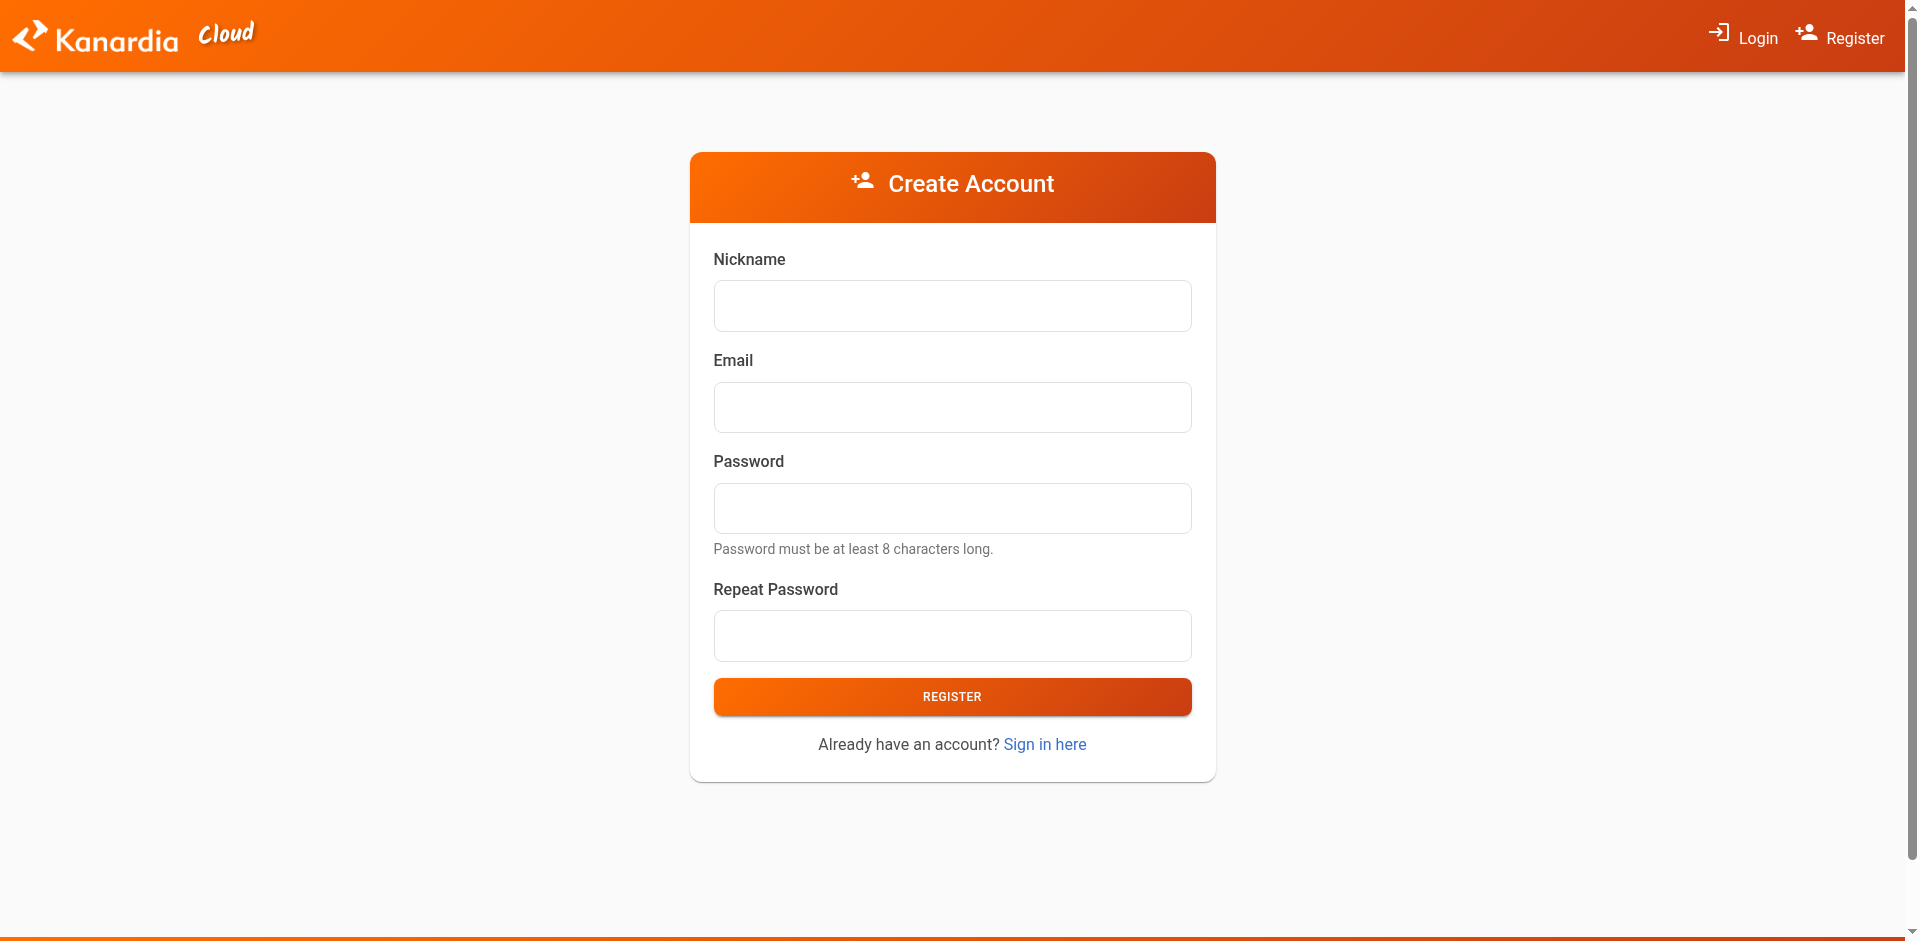
\includegraphics[width=0.8\textwidth]{images/registration_form.png}
\caption{Account Registration Form}
\label{fig:registration_form}
\end{figure}

\subsection{First Login}

After account verification:

\begin{enumerate}
    \item Return to the KanardiaCloud login page
    \item Enter your email address and password
    \item Click \textbf{"Sign In"}
    \item Complete the initial setup wizard (if prompted)
\end{enumerate}

\section{Dashboard Overview}

Upon successful login, you'll be greeted with the KanardiaCloud dashboard, which serves as your central command center.

\begin{figure}[H]
\centering
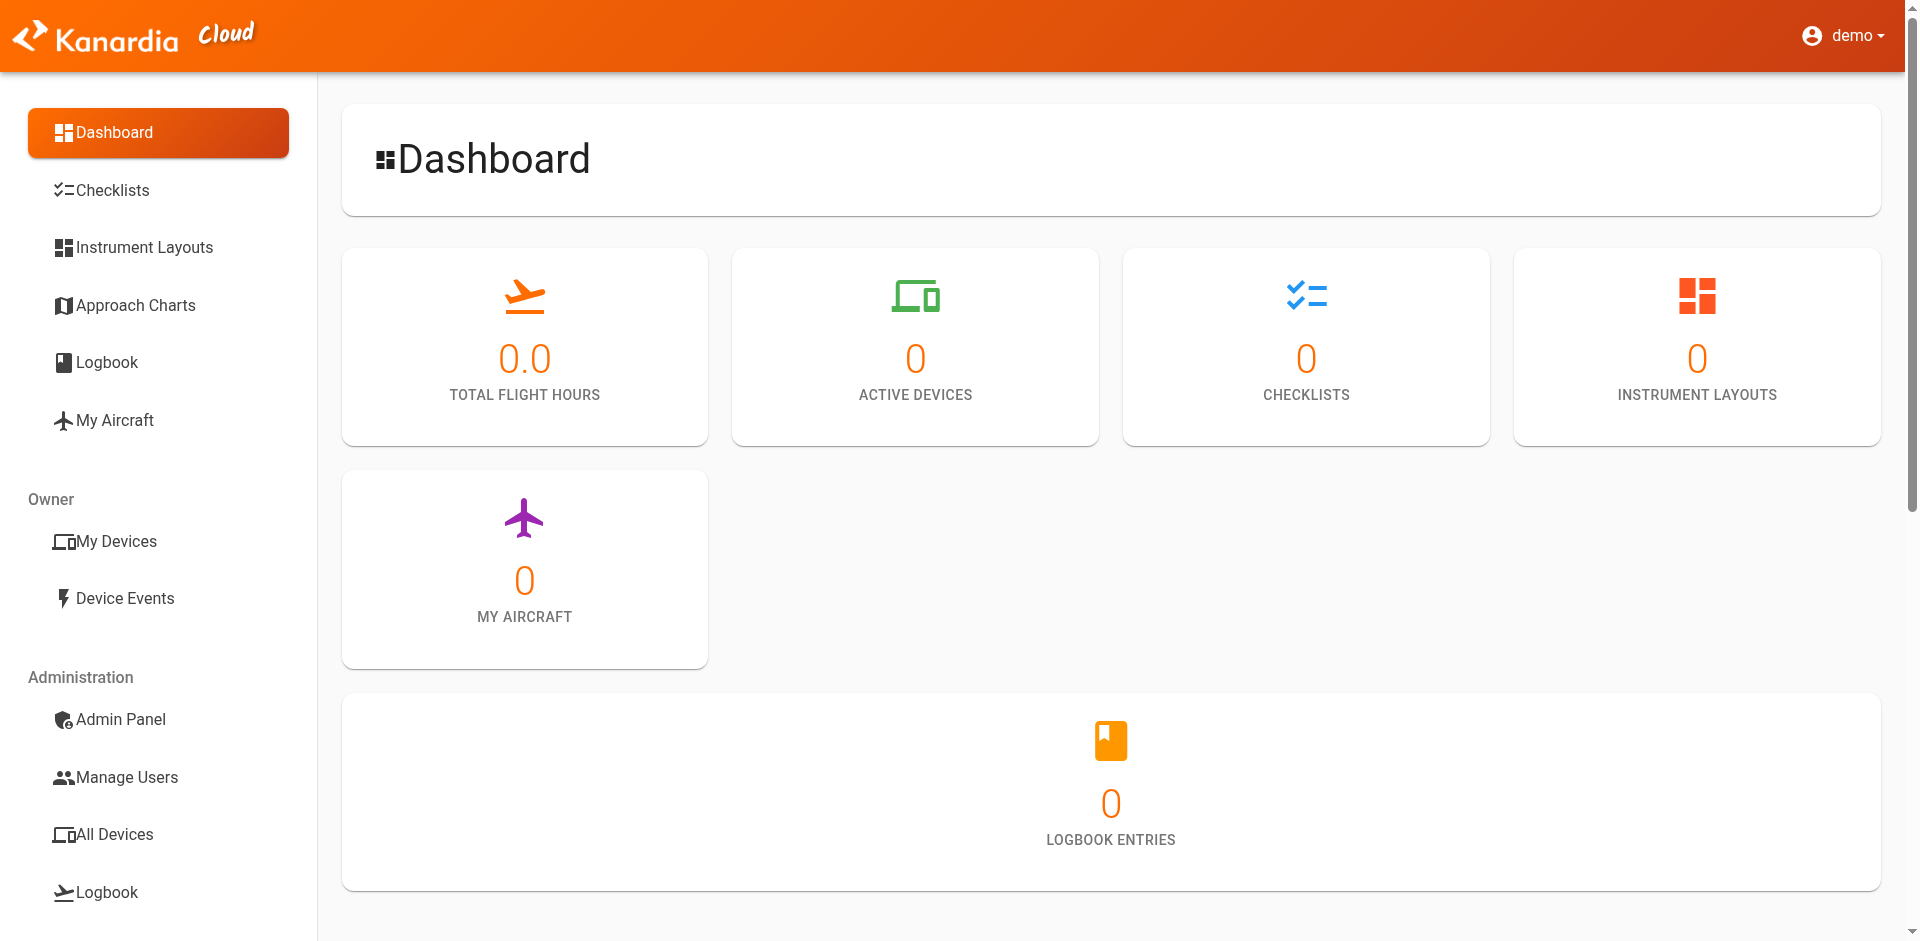
\includegraphics[width=\textwidth]{images/dashboard_overview.png}
\caption{KanardiaCloud Dashboard Overview}
\label{fig:dashboard_overview}
\end{figure}

\subsection{Navigation Menu}

The main navigation menu provides access to all KanardiaCloud features:

\begin{table}[H]
\centering
\begin{tabular}{@{}lp{8cm}@{}}
\toprule
\textbf{Menu Item} & \textbf{Description} \\
\midrule
Dashboard & Main overview with key metrics and recent activity \\
Devices & Manage and sync with Kanardia aviation devices \\
Checklists & Create, edit, and organize digital flight checklists \\
Instrument Layouts & Design custom instrument panel configurations \\
Logbook & Electronic flight logbook with automatic entries \\
Approach Charts & Store and manage airport approach procedures \\
Settings & User preferences and account configuration \\
\bottomrule
\end{tabular}
\caption{Main Navigation Menu Items}
\label{tab:navigation_menu}
\end{table}

\subsection{Quick Actions}

The dashboard provides quick access to common tasks:

\begin{itemize}
    \item \textbf{Add New Device}: Connect a new Kanardia device
    \item \textbf{Create Checklist}: Start building a new flight checklist
    \item \textbf{New Logbook Entry}: Manually add a flight record
    \item \textbf{Upload Chart}: Add new approach charts
\end{itemize}

\section{User Interface Elements}

\subsection{Common Controls}

KanardiaCloud uses consistent interface elements throughout the application:

\begin{description}
    \item[Primary Buttons] Orange buttons for main actions (Create, Save, Submit)
    \item[Secondary Buttons] Gray buttons for alternative actions (Cancel, Back)
    \item[Icon Buttons] Small buttons with icons for quick actions
    \item[Form Fields] Input fields with validation and error messages
    \item[Data Tables] Sortable and filterable tables for data display
\end{description}

\subsection{Status Indicators}

Various status indicators help you understand system states:

\begin{itemize}
    \item \textcolor{green}{\textbf{Green}}: Active, online, or successful states
    \item \textcolor{orange}{\textbf{Orange}}: Warning or attention required
    \item \textcolor{red}{\textbf{Red}}: Error, offline, or critical states
    \item \textcolor{gray}{\textbf{Gray}}: Inactive, disabled, or neutral states
\end{itemize}

\section{Basic Navigation}

\subsection{Moving Between Sections}

\begin{itemize}
    \item Use the main navigation menu on the left side
    \item Click the KanardiaCloud logo to return to the dashboard
    \item Use breadcrumb navigation for nested pages
    \item Browser back/forward buttons work as expected
\end{itemize}

\subsection{Searching and Filtering}

Most data views include search and filter capabilities:

\begin{enumerate}
    \item Look for the search box (usually in the top-right of data tables)
    \item Enter keywords to filter results in real-time
    \item Use dropdown filters for specific criteria
    \item Clear filters by clicking the "Clear" or "Reset" button
\end{enumerate}

\section{Getting Support}

\subsection{In-App Help}

\begin{itemize}
    \item Look for help icons (\texttt{?}) next to form fields
    \item Hover over tooltips for additional information
    \item Check the status bar for helpful hints
\end{itemize}

\subsection{Keyboard Shortcuts}

Common keyboard shortcuts available throughout the application:

\begin{table}[H]
\centering
\begin{tabular}{@{}ll@{}}
\toprule
\textbf{Shortcut} & \textbf{Action} \\
\midrule
Ctrl + S & Save current form or changes \\
Ctrl + N & Create new item (context-dependent) \\
Ctrl + F & Focus search field \\
Esc & Cancel current action or close modal \\
Tab & Navigate between form fields \\
\bottomrule
\end{tabular}
\caption{Keyboard Shortcuts}
\label{tab:keyboard_shortcuts}
\end{table}

\section{Initial Configuration}

\subsection{User Profile Setup}

Before using KanardiaCloud extensively, configure your user profile:

\begin{enumerate}
    \item Navigate to \textbf{Settings} $\rightarrow$ \textbf{User Profile}
    \item Update your personal information
    \item Set your preferred date/time format
    \item Configure notification preferences
    \item Set your default timezone
\end{enumerate}

\subsection{Device Connection}

If you have Kanardia devices to connect:

\begin{enumerate}
    \item Go to \textbf{Devices} section
    \item Click \textbf{"Add New Device"}
    \item Follow the device-specific setup wizard
    \item Test the connection
    \item Configure sync preferences
\end{enumerate}

\subsection{Data Import}

If you have existing flight data to import:

\begin{enumerate}
    \item Navigate to the appropriate section (Logbook, Checklists, etc.)
    \item Look for \textbf{"Import"} options
    \item Follow the import wizard
    \item Review and confirm imported data
\end{enumerate}

\chapter{Dashboard}

\section{Dashboard Overview}

The KanardiaCloud dashboard serves as your central control center, providing an at-a-glance view of all important information and quick access to frequently used features.

\begin{figure}[H]
\centering
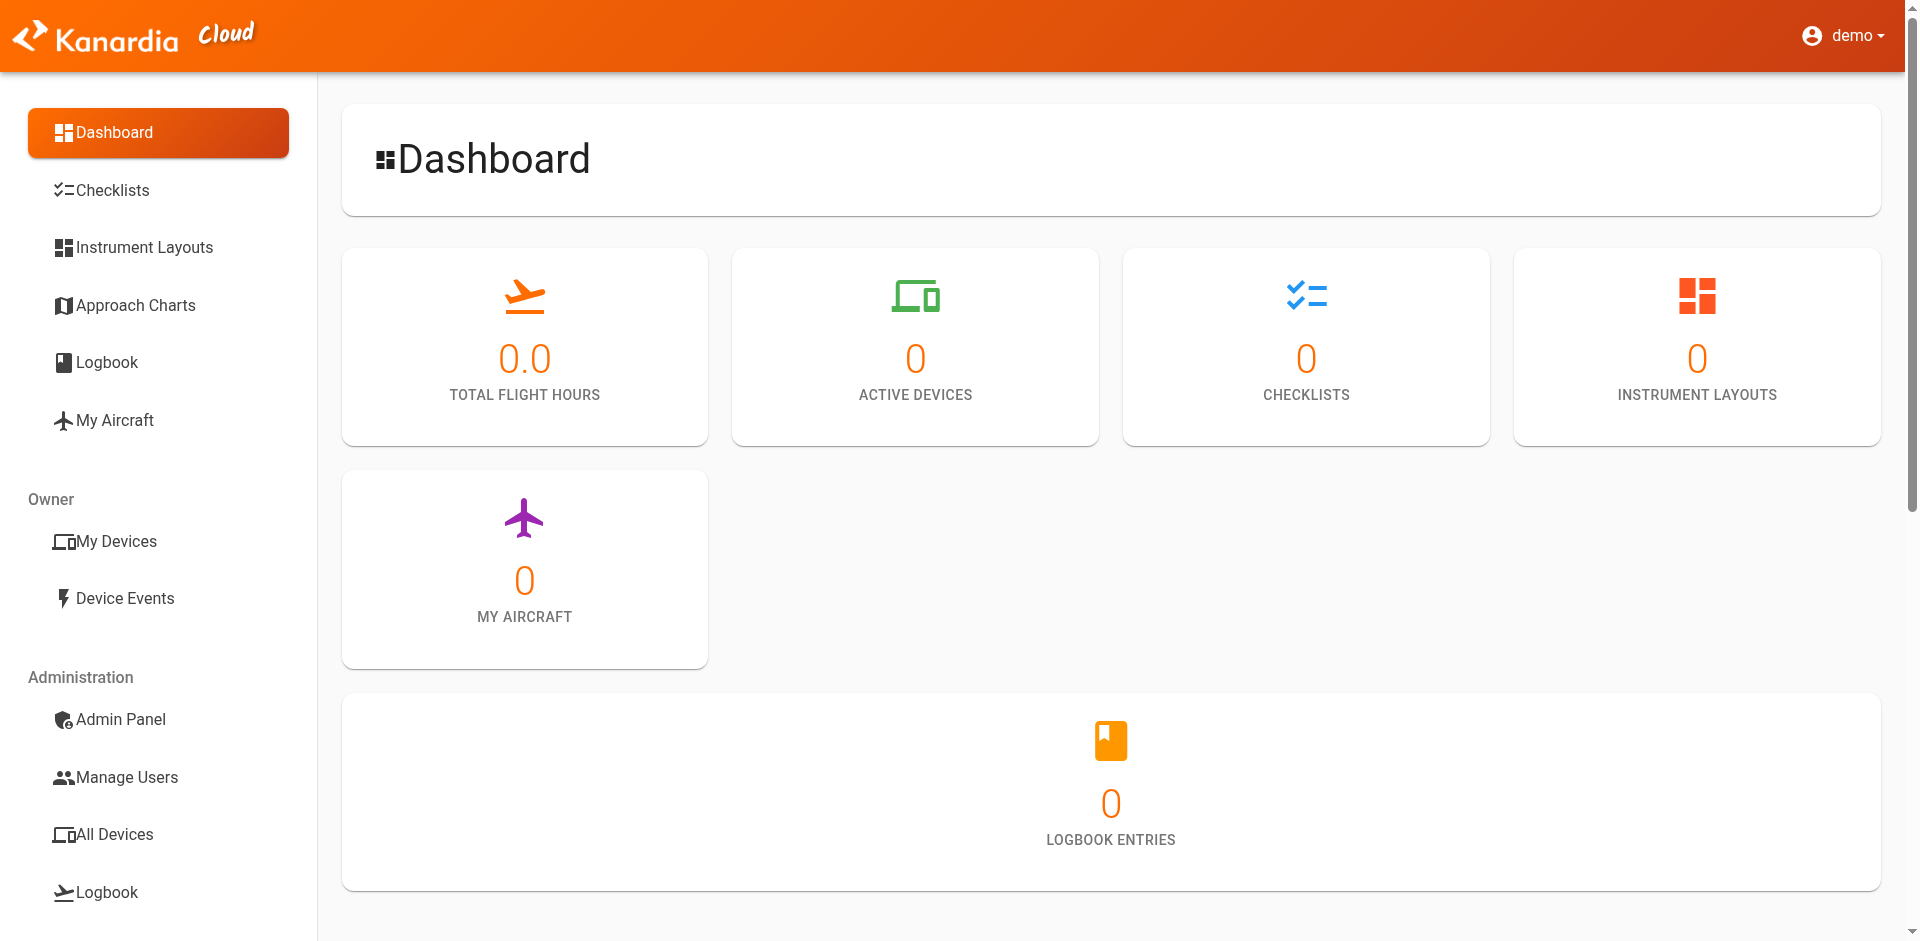
\includegraphics[width=\textwidth]{images/main_dashboard.png}
\caption{KanardiaCloud Main Dashboard}
\label{fig:main_dashboard}
\end{figure}

\section{Dashboard Components}

\subsection{Header Navigation}

The top header contains:

\begin{itemize}
    \item \textbf{Logo}: Click to return to dashboard
    \item \textbf{Main Navigation}: Access all major sections
    \item \textbf{User Menu}: Profile, settings, and logout options
    \item \textbf{Notifications}: System alerts and updates
\end{itemize}

\subsection{Quick Statistics}

Key metrics displayed prominently:

\begin{table}[H]
\centering
\begin{tabular}{@{}lp{8cm}@{}}
\toprule
\textbf{Metric} & \textbf{Description} \\
\midrule
Connected Devices & Number of active Kanardia devices \\
Total Flight Hours & Cumulative flight time from logbook \\
Active Checklists & Number of available checklists \\
Recent Flights & Last 7 days flight activity \\
System Status & Overall system health indicator \\
\bottomrule
\end{tabular}
\caption{Dashboard Quick Statistics}
\label{tab:dashboard_stats}
\end{table}

\subsection{Recent Activity}

The activity feed shows:
\begin{itemize}
    \item Recent logbook entries
    \item Checklist modifications
    \item Device synchronization events
    \item System notifications
    \item User actions and changes
\end{itemize}

\subsection{Quick Actions Panel}

One-click access to common tasks:
\begin{itemize}
    \item Add new flight entry
    \item Create checklist
    \item Connect new device
    \item Upload approach chart
    \item Generate reports
\end{itemize}

\section{Customization}

\subsection{Widget Configuration}

Customize your dashboard by:
\begin{enumerate}
    \item Clicking the settings icon in the top-right
    \item Selecting which widgets to display
    \item Arranging widget order
    \item Setting refresh intervals
    \item Configuring data ranges
\end{enumerate}

\subsection{Personal Preferences}

Set your preferences for:
\begin{itemize}
    \item Default date/time formats
    \item Measurement units (metric/imperial)
    \item Language settings
    \item Theme preferences
    \item Notification settings
\end{itemize}

\chapter{Device Management}

\section{Overview}

The Device Management system allows you to connect, configure, and synchronize data with Kanardia aviation devices. This enables automatic data collection and seamless integration between your aircraft systems and KanardiaCloud.

\section{Supported Devices}

KanardiaCloud supports various Kanardia devices:

\begin{table}[H]
\centering
\begin{tabular}{@{}llp{6cm}@{}}
\toprule
\textbf{Device} & \textbf{Type} & \textbf{Capabilities} \\
\midrule
NESIS III & Flight Management & GPS tracking, flight planning, logbook \\
NESIS IV & Flight Computer & Advanced flight management, weather \\
KRT2 S & VHF Radio & Communication logs, frequency data \\
KTX2 & Transponder & Mode S data, traffic information \\
\bottomrule
\end{tabular}
\caption{Supported Kanardia Devices}
\label{tab:supported_devices}
\end{table}

\section{Adding Devices}

\subsection{Device Registration}

To add a new device:

\begin{enumerate}
    \item Navigate to \textbf{Devices}
    \item Click \textbf{"Add New Device"}
    \item Select device type
    \item Enter device identification details
    \item Configure connection settings
    \item Test connection
    \item Complete setup wizard
\end{enumerate}

\section{Device Synchronization}

\subsection{Automatic Sync}

Devices synchronize automatically:
\begin{itemize}
    \item Flight data and logbook entries
    \item GPS tracks and waypoints
    \item System configurations
    \item Usage statistics
\end{itemize}

\subsection{Manual Sync}

Force synchronization when needed:
\begin{enumerate}
    \item Select device from list
    \item Click \textbf{"Sync Now"}
    \item Monitor sync progress
    \item Review sync results
\end{enumerate}

\chapter{Checklist Management}

\section{Overview}

The Checklist Management system in KanardiaCloud allows pilots and aviation professionals to create, organize, and print professional digital checklists. These checklists can be synchronized with Kanardia devices and printed in various formats for cockpit use.

\begin{figure}[H]
\centering
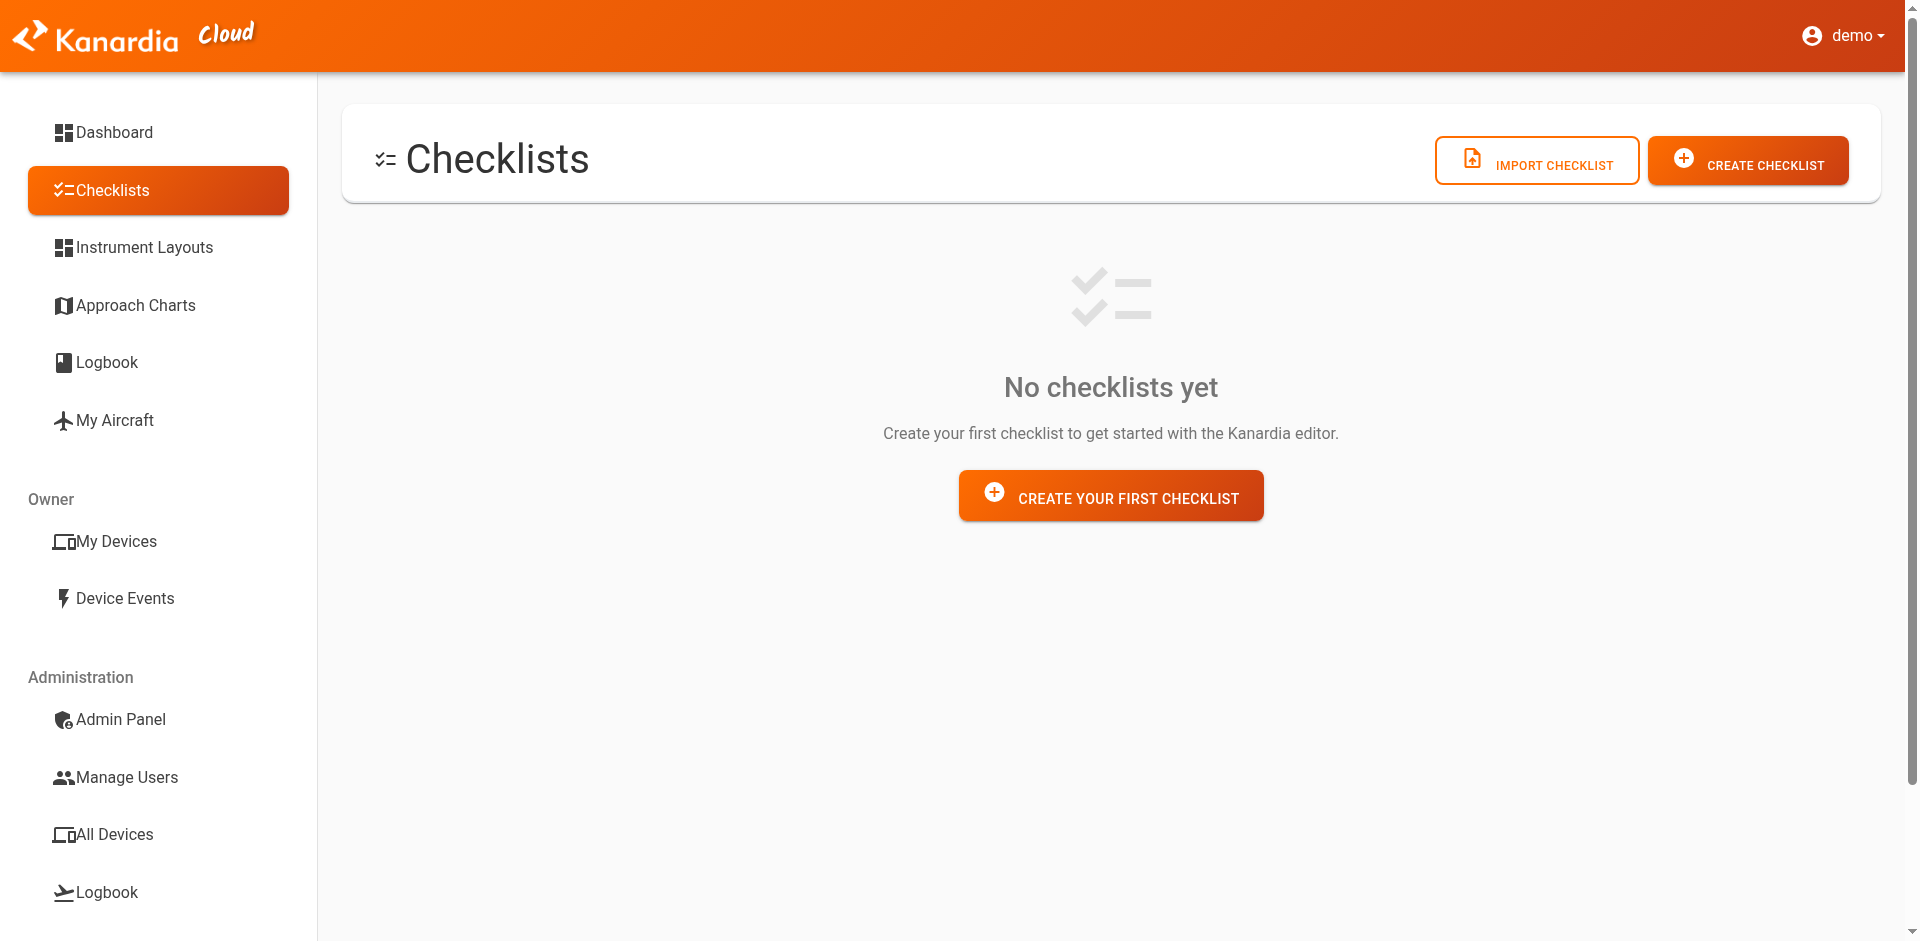
\includegraphics[width=\textwidth]{images/checklist_dashboard.png}
\caption{Checklist Management Dashboard}
\label{fig:checklist_dashboard}
\end{figure}

\section{Creating Checklists}

\subsection{New Checklist Creation}

To create a new checklist:

\begin{enumerate}
    \item Navigate to \textbf{Checklists} in the main menu
    \item Click the \textbf{"Create New Checklist"} button
    \item Fill in the basic information:
    \begin{itemize}
        \item \textbf{Title}: Descriptive name for the checklist
        \item \textbf{Description}: Optional detailed description
        \item \textbf{Aircraft Type}: Associated aircraft model (if applicable)
    \end{itemize}
    \item Click \textbf{"Create Checklist"} to proceed to the editor
\end{enumerate}

\begin{figure}[H]
\centering
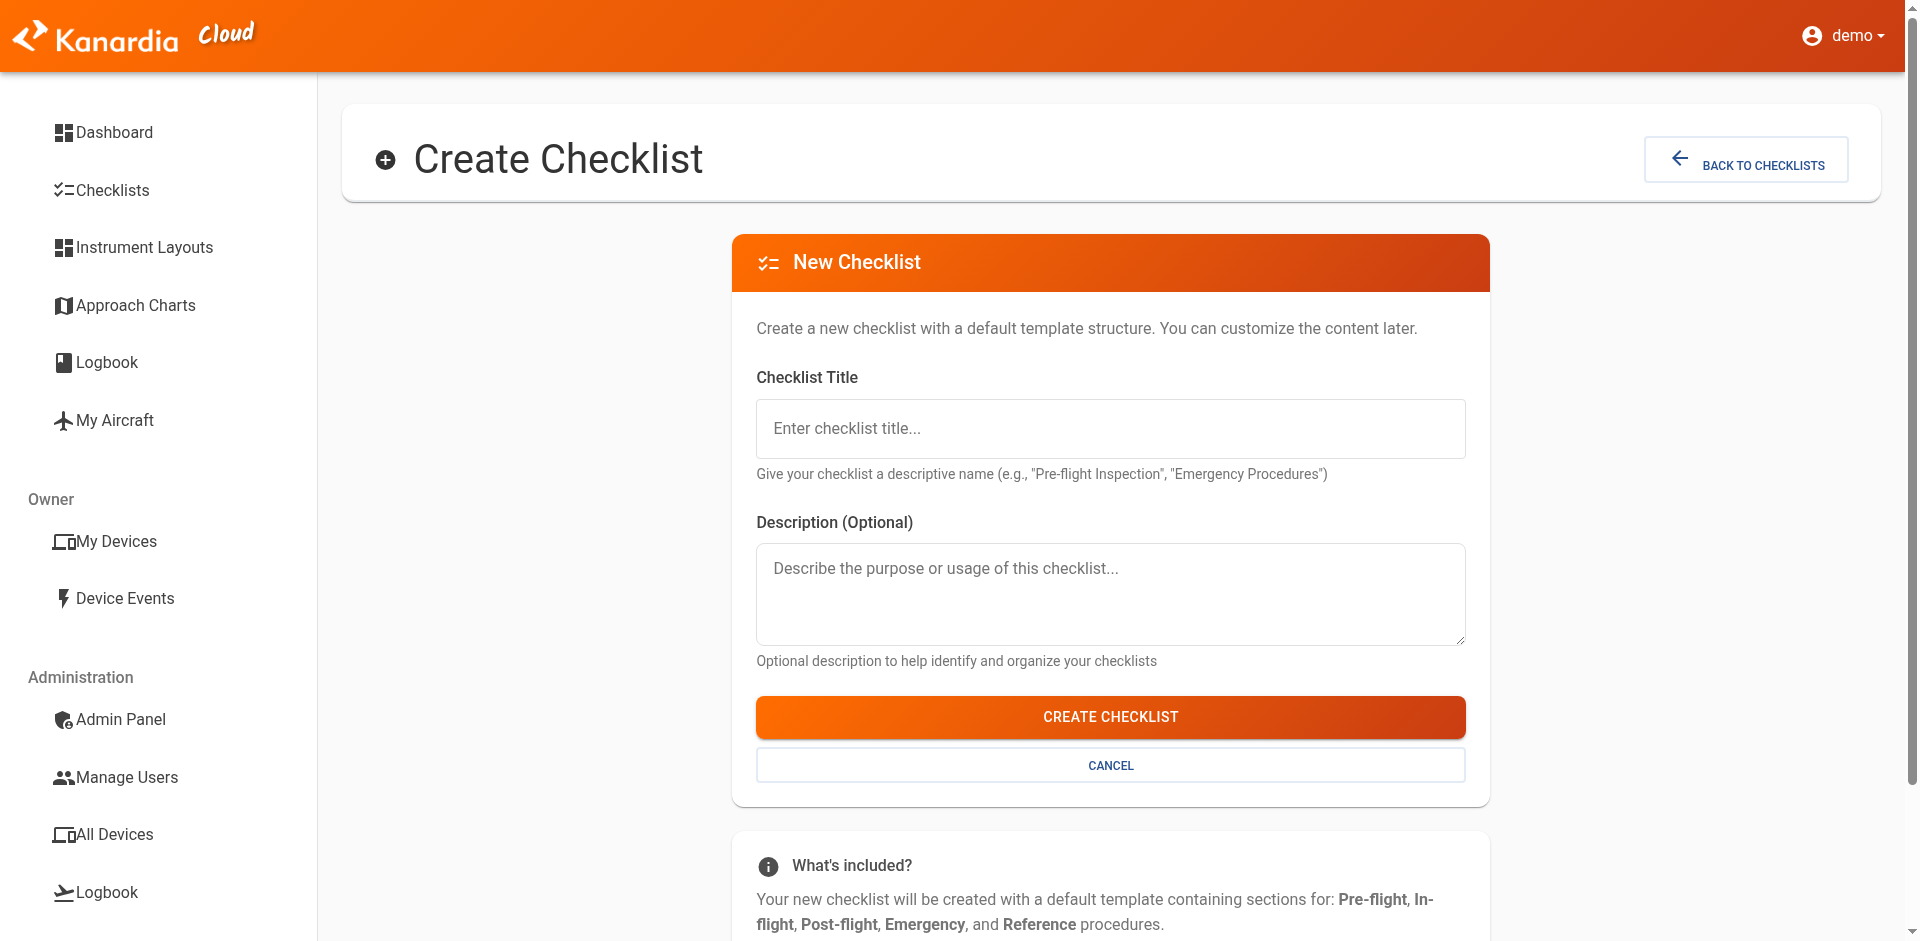
\includegraphics[width=0.8\textwidth]{images/create_checklist_form.png}
\caption{New Checklist Creation Form}
\label{fig:create_checklist_form}
\end{figure}

\subsection{Checklist Structure}

KanardiaCloud checklists are organized hierarchically:

\begin{description}
    \item[Root] Top-level container for the entire checklist
    \item[Sections] Major groupings (e.g., "Pre-flight", "Engine Start", "Landing")
    \item[Checklists] Individual procedures within sections
    \item[Items] Specific actions or checks within each checklist
\end{description}

\section{Checklist Editor}

\subsection{Editor Interface}

The checklist editor provides a comprehensive interface for building detailed checklists:

\begin{itemize}
    \item \textbf{Tree View}: Hierarchical structure on the left
    \item \textbf{Properties Panel}: Item details on the right
    \item \textbf{Toolbar}: Quick actions and tools
    \item \textbf{Preview}: Real-time preview of changes
\end{itemize}

\begin{figure}[H]
\centering

\includegraphics[width=\textwidth]{images/checklist_editor.png}
\caption{Checklist Editor Interface}
\label{fig:checklist_editor}
\end{figure}

\subsection{Adding Sections and Items}

To add new elements to your checklist:

\begin{enumerate}
    \item \textbf{Adding a Section}:
    \begin{itemize}
        \item Right-click on the root node or use the "Add Section" button
        \item Enter the section name (e.g., "Pre-flight Inspection")
        \item Set section properties if needed
    \end{itemize}
    
    \item \textbf{Adding a Checklist}:
    \begin{itemize}
        \item Right-click on a section or use "Add Checklist"
        \item Name the checklist (e.g., "External Inspection")
        \item Configure checklist properties
    \end{itemize}
    
    \item \textbf{Adding Items}:
    \begin{itemize}
        \item Right-click on a checklist or use "Add Item"
        \item Enter the item title and action
        \item Set item properties and responses
    \end{itemize}
\end{enumerate}

\subsection{Item Properties}

Each checklist item can be configured with:

\begin{table}[H]
\centering
\begin{tabular}{@{}lp{8cm}@{}}
\toprule
\textbf{Property} & \textbf{Description} \\
\midrule
Title & The main text of the checklist item \\
Action & Expected response or action to take \\
Type & Item type (check, action, warning, etc.) \\
Priority & Item importance level \\
Notes & Additional information or remarks \\
Voice & Text-to-speech pronunciation guide \\
\bottomrule
\end{tabular}
\caption{Checklist Item Properties}
\label{tab:item_properties}
\end{table}

\section{Checklist Import and Export}

\subsection{Supported Formats}

KanardiaCloud supports various checklist formats:

\begin{itemize}
    \item \textbf{Kanardia CKL}: Native Kanardia checklist format
    \item \textbf{JSON}: Standard JSON format for data exchange
    \item \textbf{XML}: Structured XML format
    \item \textbf{CSV}: Simple comma-separated values (basic import only)
\end{itemize}

\subsection{Importing Checklists}

To import an existing checklist:

\begin{enumerate}
    \item Go to \textbf{Checklists} $\rightarrow$ \textbf{Import}
    \item Select the file format
    \item Choose the checklist file
    \item Review the import preview
    \item Confirm the import
    \item Edit as needed using the checklist editor
\end{enumerate}

\begin{figure}[H]
\centering
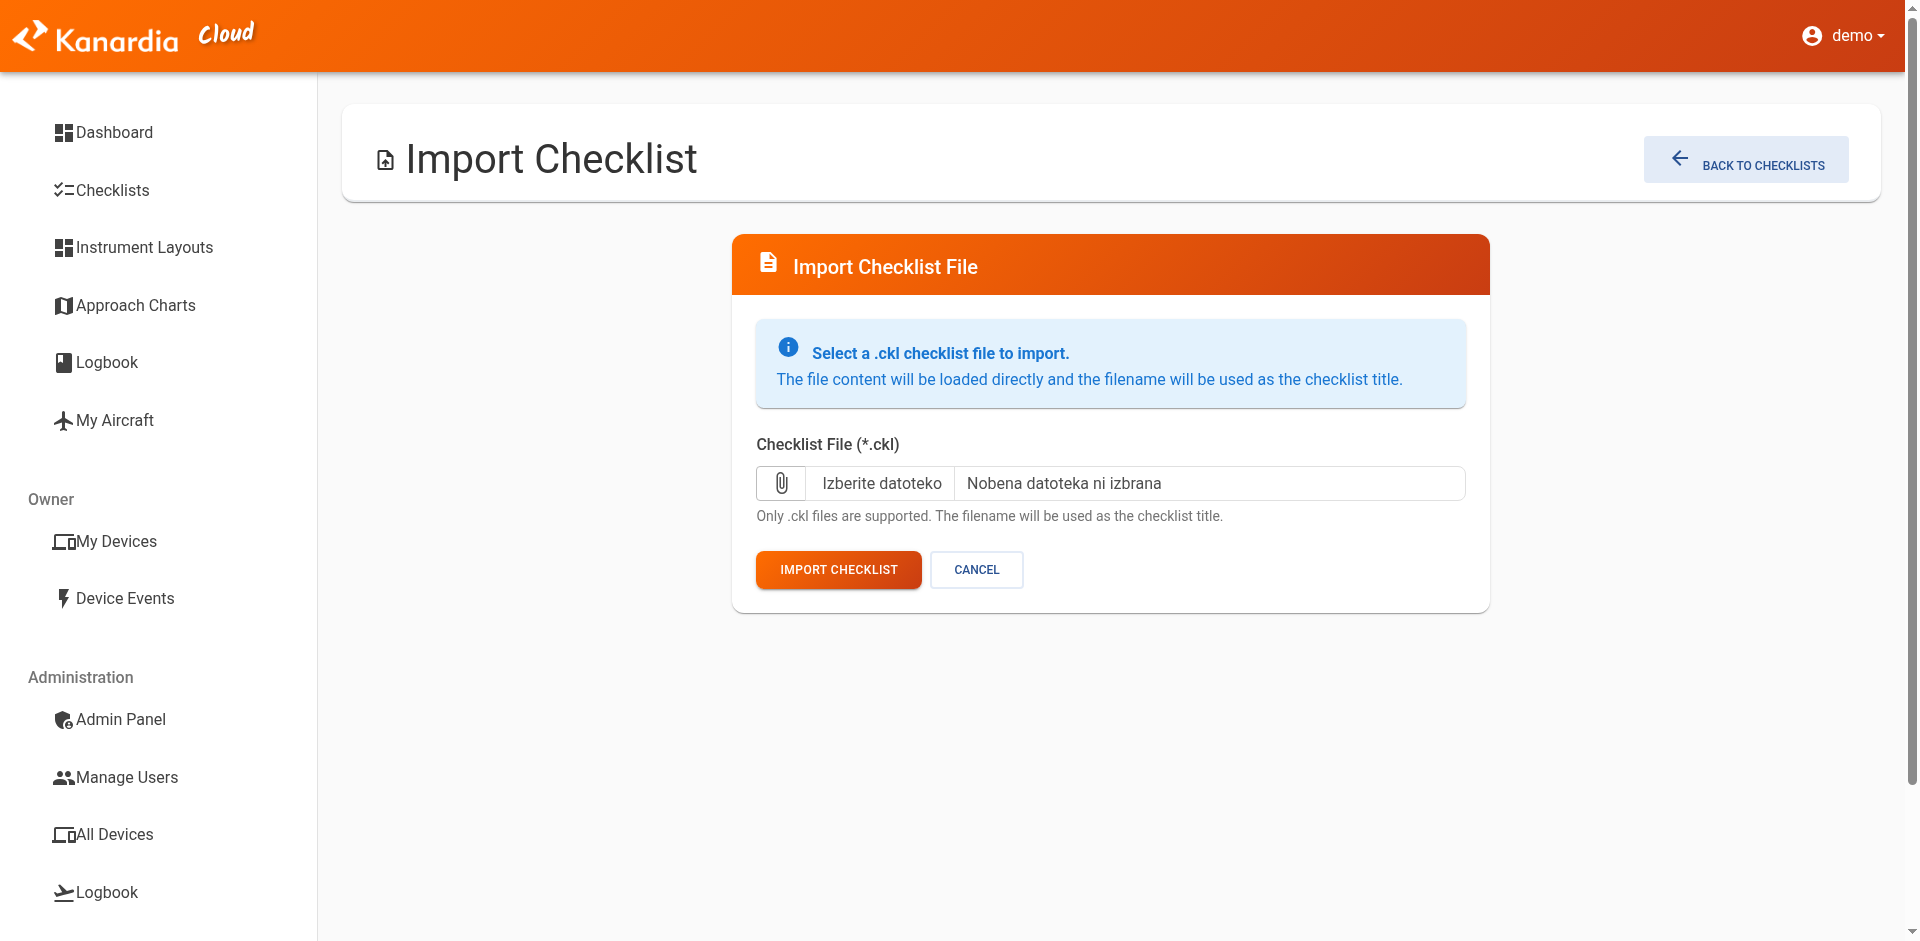
\includegraphics[width=0.8\textwidth]{images/checklist_import.png}
\caption{Checklist Import Interface}
\label{fig:checklist_import}
\end{figure}

\subsection{Exporting Checklists}

To export a checklist:

\begin{enumerate}
    \item Open the checklist you want to export
    \item Click the \textbf{"Export"} button in the toolbar
    \item Select the desired format
    \item Choose export options
    \item Download the exported file
\end{enumerate}

\section{Printable Checklists}

\subsection{Print Formats}

KanardiaCloud offers two optimized print formats:

\subsubsection{Standard Format}
\begin{itemize}
    \item Full page layout with headers and metadata
    \item Section titles prominently displayed
    \item Two-column layout for efficient paper use
    \item Complete checklist information included
\end{itemize}

\subsubsection{Minimal Format}
\begin{itemize}
    \item Compact layout without headers
    \item All checklists on one page
    \item Section names shown on each card
    \item Optimized for cockpit reference
\end{itemize}

\begin{figure}[H]
\centering
\begin{subfigure}[b]{0.48\textwidth}

\includegraphics[width=\textwidth]{images/checklist_print_standard.png}
\caption{Standard Print Format}
\label{fig:print_standard}
\end{subfigure}
\hfill
\begin{subfigure}[b]{0.48\textwidth}

\includegraphics[width=\textwidth]{images/checklist_print_minimal.png}
\caption{Minimal Print Format}
\label{fig:print_minimal}
\end{subfigure}
\caption{Checklist Print Formats}
\label{fig:print_formats}
\end{figure}

\subsection{Accessing Print Versions}

To generate printable checklists:

\begin{enumerate}
    \item Navigate to your checklist
    \item Click the options menu (three dots)
    \item Select \textbf{"Printable Version"}
    \item Choose between Standard or Minimal format
    \item Use browser print function or click \textbf{"Print Checklist"}
\end{enumerate}

\subsection{Print Optimization}

Both print formats are optimized for:
\begin{itemize}
    \item Standard A4 and Letter paper sizes
    \item Two-column layout for space efficiency
    \item Clear, readable fonts suitable for cockpit lighting
    \item Professional appearance with Kanardia branding
    \item Page breaks that avoid splitting checklists
\end{itemize}

\section{Checklist Organization}

\subsection{Categories and Tagging}

Organize your checklists using:

\begin{itemize}
    \item \textbf{Categories}: Group by aircraft type, operation type, etc.
    \item \textbf{Tags}: Custom labels for flexible organization
    \item \textbf{Favorites}: Mark frequently used checklists
    \item \textbf{Recent}: Quick access to recently modified items
\end{itemize}

\subsection{Search and Filtering}

Find checklists quickly using:

\begin{itemize}
    \item \textbf{Text Search}: Search titles and content
    \item \textbf{Category Filters}: Filter by assigned categories
    \item \textbf{Date Filters}: Show recently created or modified
    \item \textbf{Status Filters}: Filter by completion or approval status
\end{itemize}

\section{Collaboration and Sharing}

\subsection{Sharing Checklists}

Share checklists with team members:

\begin{enumerate}
    \item Open the checklist to share
    \item Click \textbf{"Share"} in the toolbar
    \item Enter recipient email addresses
    \item Set permission levels (view, edit, admin)
    \item Add an optional message
    \item Click \textbf{"Send Invitation"}
\end{enumerate}

\subsection{Version Control}

KanardiaCloud maintains checklist versions:

\begin{itemize}
    \item Automatic version history
    \item Compare different versions
    \item Restore previous versions
    \item Track changes and modifications
    \item Comment on changes
\end{itemize}

\section{Best Practices}

\subsection{Checklist Design}

Follow these guidelines for effective checklists:

\begin{itemize}
    \item \textbf{Clear Language}: Use precise, unambiguous terms
    \item \textbf{Logical Flow}: Arrange items in operational sequence
    \item \textbf{Consistent Format}: Maintain uniform structure
    \item \textbf{Appropriate Length}: Keep individual checklists manageable
    \item \textbf{Regular Updates}: Review and update periodically
\end{itemize}

\subsection{Naming Conventions}

Use consistent naming for easy identification:

\begin{itemize}
    \item Include aircraft type in title
    \item Use standard aviation terminology
    \item Follow company or organizational standards
    \item Include version numbers or dates
\end{itemize}

\subsection{Testing and Validation}

Before using checklists operationally:

\begin{itemize}
    \item Review with experienced pilots
    \item Test in simulator environments
    \item Validate against official procedures
    \item Check for completeness and accuracy
    \item Obtain necessary approvals
\end{itemize}

\section{Troubleshooting}

\subsection{Common Issues}

\begin{description}
    \item[Import Failures] Check file format and encoding, ensure file is not corrupted
    \item[Print Layout Issues] Verify browser print settings, try different browsers
    \item[Sync Problems] Check device connection, verify account permissions
    \item[Missing Items] Refresh page, check filter settings, verify data integrity
\end{description}

\subsection{Getting Help}

If you encounter issues with checklist management:

\begin{itemize}
    \item Check the built-in help tooltips
    \item Review this user manual
    \item Contact support with specific error messages
    \item Provide checklist files for technical analysis
\end{itemize}

\chapter{Instrument Layouts}

\section{Overview}

The Instrument Layout system allows you to design and configure custom instrument panel arrangements for different aircraft or flight scenarios. These layouts can be synchronized with compatible Kanardia displays.

\section{Creating Layouts}

\subsection{New Layout Wizard}

To create a new instrument layout:

\begin{enumerate}
    \item Navigate to \textbf{Instrument Layouts}
    \item Click \textbf{"Create New Layout"}
    \item Enter layout details:
    \begin{itemize}
        \item Title and description
        \item Aircraft type or model
        \item Display resolution
        \item Layout category
    \end{itemize}
    \item Choose from templates or start blank
    \item Proceed to the layout editor
\end{enumerate}

\section{Layout Editor}

\subsection{Editor Interface}

The layout editor provides:
\begin{itemize}
    \item Drag-and-drop instrument placement
    \item Real-time preview
    \item Instrument property configuration
    \item Grid snapping and alignment tools
    \item Zoom and pan controls
\end{itemize}

\subsection{Available Instruments}

Standard instrument types include:
\begin{itemize}
    \item Primary flight display components
    \item Engine monitoring instruments
    \item Navigation displays
    \item Communication panels
    \item Custom gauges and indicators
\end{itemize}

\section{Layout Management}

\subsection{Organization}

Organize layouts by:
\begin{itemize}
    \item Aircraft type
    \item Flight phase
    \item User preference
    \item Certification level
\end{itemize}

\subsection{Sharing and Export}

Share layouts with:
\begin{itemize}
    \item Team members
    \item Aircraft operators
    \item Training organizations
    \item Device synchronization
\end{itemize}

\chapter{Electronic Logbook}

\section{Overview}

The Electronic Logbook system automatically records and manages flight data from connected Kanardia devices, providing comprehensive flight tracking and regulatory compliance features.

\section{Logbook Entries}

\subsection{Automatic Entry Creation}

Flight entries are created automatically when:
\begin{itemize}
    \item Aircraft engines start
    \item GPS tracking begins
    \item Flight parameters exceed thresholds
    \item Landing is detected
\end{itemize}

\subsection{Manual Entry Creation}

Add manual entries for:
\begin{itemize}
    \item Training flights
    \item Ground instruction
    \item Simulator sessions
    \item Non-connected aircraft
\end{itemize}

\section{Data Fields}

\subsection{Standard Fields}

Each logbook entry includes:

\begin{table}[H]
\centering
\begin{tabular}{@{}lp{8cm}@{}}
\toprule
\textbf{Field} & \textbf{Description} \\
\midrule
Date & Flight date \\
Aircraft & Aircraft registration and type \\
Departure & Origin airport and time \\
Arrival & Destination airport and time \\
Flight Time & Total flight duration \\
Pilot in Command & PIC identification \\
Remarks & Additional notes and comments \\
\bottomrule
\end{tabular}
\caption{Standard Logbook Fields}
\label{tab:logbook_fields}
\end{table}

\subsection{Extended Data}

Additional information captured:
\begin{itemize}
    \item GPS flight tracks
    \item Engine parameters
    \item Weather conditions
    \item Fuel consumption
    \item Performance metrics
\end{itemize}

\section{Reports and Analysis}

\subsection{Flight Reports}

Generate various reports:
\begin{itemize}
    \item Individual flight summaries
    \item Monthly/yearly totals
    \item Aircraft utilization
    \item Maintenance tracking
    \item Regulatory compliance
\end{itemize}

\subsection{Export Options}

Export data in formats:
\begin{itemize}
    \item PDF reports
    \item Excel spreadsheets
    \item CSV data files
    \item Standard logbook formats
\end{itemize}

\chapter{Approach Charts}

\section{Overview}

The Approach Charts system allows you to store, organize, and access airport approach procedures and charts. These can be synchronized with compatible Kanardia navigation systems for in-flight reference.

\section{Chart Management}

\subsection{Uploading Charts}

To add new approach charts:

\begin{enumerate}
    \item Navigate to \textbf{Approach Charts}
    \item Click \textbf{"Upload Chart"}
    \item Select chart file (PDF, PNG, JPG supported)
    \item Enter chart information:
    \begin{itemize}
        \item Airport identifier
        \item Approach type
        \item Runway designation
        \item Effective dates
    \end{itemize}
    \item Verify chart preview
    \item Save chart to library
\end{enumerate}

\subsection{Chart Organization}

Organize charts by:
\begin{itemize}
    \item Airport or region
    \item Approach type (ILS, RNAV, VOR, etc.)
    \item Currency status
    \item Frequency of use
\end{itemize}

\section{Chart Access}

\subsection{Search and Filter}

Find charts quickly using:
\begin{itemize}
    \item Airport identifier search
    \item Approach type filters
    \item Geographic region filters
    \item Date range filters
\end{itemize}

\subsection{Chart Viewing}

View charts with features:
\begin{itemize}
    \item Zoom and pan controls
    \item Full-screen mode
    \item Rotation and orientation
    \item Annotation tools
\end{itemize}

\section{Integration}

\subsection{Device Synchronization}

Sync charts with:
\begin{itemize}
    \item NESIS displays
    \item Portable devices
    \item Flight planning systems
    \item Navigation databases
\end{itemize}

\chapter{User Settings}

\section{Profile Management}

\subsection{Personal Information}

Manage your profile settings:

\begin{itemize}
    \item Full name and contact information
    \item Professional licenses and ratings
    \item Organization affiliation
    \item Profile picture
\end{itemize}

\subsection{Account Security}

Configure security settings:

\begin{itemize}
    \item Password management
    \item Two-factor authentication
    \item Login session management
    \item Security notification preferences
\end{itemize}

\section{Display Preferences}

\subsection{Regional Settings}

Customize regional preferences:

\begin{table}[H]
\centering
\begin{tabular}{@{}ll@{}}
\toprule
\textbf{Setting} & \textbf{Options} \\
\midrule
Date Format & DD/MM/YYYY, MM/DD/YYYY, YYYY-MM-DD \\
Time Format & 12-hour, 24-hour \\
Units & Metric, Imperial, Mixed \\
Language & English, German, Slovenian \\
Timezone & User-selectable timezone \\
\bottomrule
\end{tabular}
\caption{Regional Settings Options}
\label{tab:regional_settings}
\end{table}

\subsection{Interface Customization}

Personalize your interface:

\begin{itemize}
    \item Theme selection (Light, Dark, Auto)
    \item Color scheme preferences
    \item Font size adjustments
    \item Dashboard widget configuration
    \item Menu organization
\end{itemize}

\section{Notification Settings}

\subsection{Email Notifications}

Configure email alerts for:

\begin{itemize}
    \item Device synchronization status
    \item System maintenance notifications
    \item Security alerts
    \item Data backup confirmations
    \item Shared content updates
\end{itemize}

\subsection{In-App Notifications}

Control in-application notifications:

\begin{itemize}
    \item Real-time sync status
    \item Error and warning messages
    \item Feature updates
    \item Tips and suggestions
\end{itemize}

\section{Data Management}

\subsection{Backup and Export}

Manage your data:

\begin{itemize}
    \item Automatic cloud backup
    \item Manual data export
    \item Selective data download
    \item Archive management
\end{itemize}

\subsection{Privacy Controls}

Control data sharing:

\begin{itemize}
    \item Data sharing preferences
    \item Third-party integrations
    \item Analytics participation
    \item Content visibility settings
\end{itemize}

\chapter{Troubleshooting}

\section{Common Issues}

\subsection{Login Problems}

\begin{description}
    \item[Forgotten Password] Use the "Forgot Password" link on login page
    \item[Account Locked] Contact support if multiple login attempts fail
    \item[Email Verification] Check spam folder for verification emails
    \item[Browser Issues] Clear cache and cookies, try different browser
\end{description}

\subsection{Device Connection Issues}

\begin{description}
    \item[Device Not Found] Verify device is powered on and connected
    \item[Sync Failures] Check network connection and device settings
    \item[Data Inconsistencies] Force full synchronization from device menu
    \item[Outdated Firmware] Update device firmware to latest version
\end{description}

\subsection{Performance Issues}

\begin{description}
    \item[Slow Loading] Check internet connection speed and stability
    \item[Browser Compatibility] Use supported browser versions
    \item[Cache Issues] Clear browser cache and refresh page
    \item[Memory Usage] Close unnecessary browser tabs and applications
\end{description}

\section{Error Messages}

\subsection{System Errors}

Common error codes and solutions:

\begin{table}[H]
\centering
\begin{tabular}{@{}lp{8cm}@{}}
\toprule
\textbf{Error Code} & \textbf{Solution} \\
\midrule
ERR\_001 & Database connection issue - try again later \\
ERR\_002 & Invalid user credentials - check login details \\
ERR\_003 & File upload failed - verify file format and size \\
ERR\_004 & Device synchronization timeout - retry sync \\
ERR\_005 & Insufficient permissions - contact administrator \\
\bottomrule
\end{tabular}
\caption{Common Error Codes}
\label{tab:error_codes}
\end{table}

\section{Getting Support}

\subsection{Self-Help Resources}

Before contacting support:

\begin{itemize}
    \item Check this user manual
    \item Review online help documentation
    \item Search the knowledge base
    \item Try suggested troubleshooting steps
\end{itemize}

\subsection{Contacting Support}

When you need assistance:

\begin{enumerate}
    \item Gather relevant information:
    \begin{itemize}
        \item Error messages or codes
        \item Steps to reproduce the issue
        \item Browser and operating system details
        \item Screenshot of the problem
    \end{itemize}
    \item Contact support via:
    \begin{itemize}
        \item Email: support@kanardia.com
        \item Phone: +386 5 365 46 70
        \item Online support portal
    \end{itemize}
    \item Provide detailed problem description
    \item Follow up on support ticket as needed
\end{enumerate}

\subsection{Emergency Support}

For critical issues affecting flight operations:

\begin{itemize}
    \item Use emergency support hotline
    \item Clearly identify safety implications
    \item Provide immediate contact information
    \item Follow emergency procedures in your organization
\end{itemize}

\section{Best Practices}

\subsection{Preventive Measures}

To minimize issues:

\begin{itemize}
    \item Keep browsers updated to latest versions
    \item Regularly backup important data
    \item Use strong, unique passwords
    \item Monitor device firmware updates
    \item Report issues promptly
\end{itemize}

\subsection{Data Recovery}

In case of data loss:

\begin{itemize}
    \item Check automatic backups
    \item Review recent sync logs
    \item Contact support immediately
    \item Avoid making changes until recovery
\end{itemize}

\chapter{API Reference}

\section{Overview}

KanardiaCloud provides a RESTful API for third-party integrations and custom applications. This chapter covers the essential API endpoints and usage examples.

\section{Authentication}

\subsection{API Key Authentication}

To access the API:

\begin{enumerate}
    \item Generate API key in user settings
    \item Include key in request headers
    \item Use HTTPS for all requests
    \item Monitor usage and rate limits
\end{enumerate}

Example request:
\begin{lstlisting}[language=bash]
curl -X GET "https://api.kanardiacloud.com/v1/devices" \
     -H "Authorization: Bearer YOUR_API_KEY" \
     -H "Content-Type: application/json"
\end{lstlisting}

\section{Core Endpoints}

\subsection{Device Management}

\begin{table}[H]
\centering
\begin{tabular}{@{}llp{6cm}@{}}
\toprule
\textbf{Method} & \textbf{Endpoint} & \textbf{Description} \\
\midrule
GET & /api/v1/devices & List all devices \\
POST & /api/v1/devices & Add new device \\
GET & /api/v1/devices/\{id\} & Get device details \\
PUT & /api/v1/devices/\{id\} & Update device \\
DELETE & /api/v1/devices/\{id\} & Remove device \\
\bottomrule
\end{tabular}
\caption{Device Management API Endpoints}
\label{tab:device_api}
\end{table}

\subsection{Logbook Management}

\begin{table}[H]
\centering
\begin{tabular}{@{}llp{6cm}@{}}
\toprule
\textbf{Method} & \textbf{Endpoint} & \textbf{Description} \\
\midrule
GET & /api/v1/logbook & List logbook entries \\
POST & /api/v1/logbook & Create new entry \\
GET & /api/v1/logbook/\{id\} & Get entry details \\
PUT & /api/v1/logbook/\{id\} & Update entry \\
DELETE & /api/v1/logbook/\{id\} & Delete entry \\
\bottomrule
\end{tabular}
\caption{Logbook API Endpoints}
\label{tab:logbook_api}
\end{table}

\subsection{Checklist Management}

\begin{table}[H]
\centering
\begin{tabular}{@{}llp{6cm}@{}}
\toprule
\textbf{Method} & \textbf{Endpoint} & \textbf{Description} \\
\midrule
GET & /api/v1/checklists & List all checklists \\
POST & /api/v1/checklists & Create new checklist \\
GET & /api/v1/checklists/\{id\} & Get checklist details \\
PUT & /api/v1/checklists/\{id\} & Update checklist \\
DELETE & /api/v1/checklists/\{id\} & Delete checklist \\
\bottomrule
\end{tabular}
\caption{Checklist API Endpoints}
\label{tab:checklist_api}
\end{table}

\section{Data Formats}

\subsection{Request/Response Format}

All API endpoints use JSON format:

\begin{lstlisting}[language=json]
{
  "success": true,
  "data": {
    "id": 123,
    "name": "Example Device",
    "status": "active",
    "lastSync": "2025-08-21T10:30:00Z"
  },
  "message": "Operation completed successfully"
}
\end{lstlisting}

\subsection{Error Handling}

Error responses include:

\begin{lstlisting}[language=json]
{
  "success": false,
  "error": {
    "code": "INVALID_REQUEST",
    "message": "Required field 'name' is missing",
    "details": {
      "field": "name",
      "required": true
    }
  }
}
\end{lstlisting}

\section{Rate Limits}

\subsection{Usage Limits}

API usage is subject to rate limits:

\begin{table}[H]
\centering
\begin{tabular}{@{}ll@{}}
\toprule
\textbf{Plan} & \textbf{Requests per Hour} \\
\midrule
Basic & 1,000 \\
Professional & 5,000 \\
Enterprise & 20,000 \\
\bottomrule
\end{tabular}
\caption{API Rate Limits}
\label{tab:rate_limits}
\end{table}

\subsection{Rate Limit Headers}

Response headers include:

\begin{itemize}
    \item \texttt{X-RateLimit-Limit}: Maximum requests allowed
    \item \texttt{X-RateLimit-Remaining}: Requests remaining in current window
    \item \texttt{X-RateLimit-Reset}: Time when limit resets
\end{itemize}

\section{SDK and Libraries}

\subsection{Official SDKs}

Kanardia provides SDKs for:

\begin{itemize}
    \item Python
    \item JavaScript/Node.js
    \item Java
    \item C\#/.NET
\end{itemize}

\subsection{Community Libraries}

Third-party libraries available for:

\begin{itemize}
    \item PHP
    \item Ruby
    \item Go
    \item Swift
\end{itemize}


% Appendices
\appendix
\chapter{Glossary and Abbreviations}

\section{Aviation Terms}

\begin{description}
    \item[AGL] Above Ground Level
    \item[AHRS] Attitude and Heading Reference System
    \item[ARINC] Aeronautical Radio, Incorporated standard
    \item[EFIS] Electronic Flight Information System
    \item[FADEC] Full Authority Digital Engine Control
    \item[FMS] Flight Management System
    \item[GNSS] Global Navigation Satellite System
    \item[IFR] Instrument Flight Rules
    \item[MSL] Mean Sea Level
    \item[RNAV] Area Navigation
    \item[VFR] Visual Flight Rules
    \item[WAAS] Wide Area Augmentation System
\end{description}

\section{Technical Terms}

\begin{description}
    \item[API] Application Programming Interface
    \item[CSV] Comma-Separated Values
    \item[HTTPS] HyperText Transfer Protocol Secure
    \item[JSON] JavaScript Object Notation
    \item[PDF] Portable Document Format
    \item[REST] Representational State Transfer
    \item[SSL] Secure Sockets Layer
    \item[TLS] Transport Layer Security
    \item[URL] Uniform Resource Locator
    \item[XML] eXtensible Markup Language
\end{description}

\section{Kanardia Terminology}

\begin{description}
    \item[CKL] Kanardia Checklist format
    \item[NESIS] Kanardia's Electronic Flight Information System
    \item[KRT2] Kanardia VHF radio transceiver
    \item[KTX2] Kanardia Mode S transponder
    \item[ThingsBoard] IoT platform used for device management
\end{description}

\chapter{File Formats and Specifications}

\section{Checklist File Formats}

\subsection{Kanardia CKL Format}

The native Kanardia checklist format uses a hierarchical structure:

\begin{lstlisting}[language=json]
{
  "Root": {
    "Children": [
      {
        "Type": 0,
        "Name": "Pre-flight",
        "Children": [
          {
            "Type": 1,
            "Name": "External Inspection",
            "Items": [
              {
                "Title": "Aircraft General Condition",
                "Action": "CHECK"
              }
            ]
          }
        ]
      }
    ]
  },
  "Language": "en-gb",
  "Voice": "Default"
}
\end{lstlisting}

\subsection{Type Definitions}

\begin{table}[H]
\centering
\begin{tabular}{@{}ll@{}}
\toprule
\textbf{Type Value} & \textbf{Element Type} \\
\midrule
0 & Section (container for checklists) \\
1 & Checklist (container for items) \\
2 & Item (individual checklist step) \\
\bottomrule
\end{tabular}
\caption{CKL Element Types}
\label{tab:ckl_types}
\end{table}

\section{Import/Export Formats}

\subsection{Supported File Types}

\begin{table}[H]
\centering
\begin{tabular}{@{}llp{6cm}@{}}
\toprule
\textbf{Format} & \textbf{Extension} & \textbf{Description} \\
\midrule
Kanardia CKL & .ckl & Native checklist format \\
JSON & .json & Standard JSON format \\
XML & .xml & Structured XML data \\
CSV & .csv & Comma-separated values \\
PDF & .pdf & Portable document (charts) \\
PNG & .png & Portable network graphics \\
JPEG & .jpg, .jpeg & Joint photographic experts group \\
\bottomrule
\end{tabular}
\caption{Supported File Formats}
\label{tab:file_formats}
\end{table}

\section{Data Schema Specifications}

\subsection{Device Data Schema}

Device information structure:

\begin{lstlisting}[language=json]
{
  "deviceId": "string",
  "name": "string",
  "type": "NESIS_III|NESIS_IV|KRT2|KTX2",
  "serialNumber": "string",
  "firmwareVersion": "string",
  "status": "active|inactive|error",
  "lastSync": "ISO 8601 datetime",
  "configuration": {
    "syncInterval": "number (minutes)",
    "dataTypes": ["logbook", "checklists", "layouts"]
  }
}
\end{lstlisting}

\subsection{Logbook Entry Schema}

Flight entry data structure:

\begin{lstlisting}[language=json]
{
  "entryId": "string",
  "date": "ISO 8601 date",
  "aircraft": {
    "registration": "string",
    "type": "string"
  },
  "departure": {
    "airport": "ICAO code",
    "time": "ISO 8601 datetime"
  },
  "arrival": {
    "airport": "ICAO code", 
    "time": "ISO 8601 datetime"
  },
  "flightTime": "number (hours)",
  "picTime": "number (hours)",
  "remarks": "string"
}
\end{lstlisting}


% Bibliography (if needed)
% \bibliography{references}
% \bibliographystyle{plain}

\end{document}
